\chapter{Machine Learning in High Energy Physics}

Machine-learning (ML) methods play an increasingly central role in high-energy-physics analyses, from low-level detector reconstruction to high-level statistical inference \cite{PhysRevD.112.016004}. Their usefulness derives from the ability to learn complex, non-linear correlations in high-dimensional feature spaces that are difficult to express in analytic form. Historically, particle physicists pioneered the use of multivariate algorithms in the 1990s and 2000s for analysis tasks, relying on techniques like artificial neural networks and boosted decision trees (BDTs) \cite{Guest_2018}. The emergence of deep learning around 2012 enabled training of very large neural networks that outperformed previous state of the art models \cite{Guest_2018}. This caused a rapid expansion of HEP applications spanning across particle/event identification, reconstruction and even real-time data filtering \cite{albertsson2019machinelearninghighenergy}.


\section{Machine Learning using Deep Neural Networks}

Neural networks (NNs) are computational models designed to approximate a mapping from input variables \textbf{x} to a desired output \textbf{y}. They consist of interconnected nodes organized into layers, inspired by the structure of the human brain \cite{hammad2024artificialneuralnetworkdeep}. The input layer contains one node for each dimension of the training data. The output layer corresponds to the desired output dimensions, reflecting the number of distinct mappings the network needs to learn. Between input and output layer, a varying number of hidden layers number enhance the network’s ability to adapt and model complex patterns. Each node is associated with a weight, a bias, and an activation function, enabling non-linear mappings for intricate problems \cite{Goodfellow-et-al-2016}. During training, a process called backpropagation adjusts these weights by computing gradients across the network from input to output, guided by a specified loss function.

When the number of hidden layers increases significantly, the network is typically referred to as a deep neural network (DNN), capable of modelling highly complex relationships in data. DNNs can approximate arbitrarily complicated functions, making them well-suited for tasks such as particle identification, energy regression, pile-up mitigation, and anomaly detection \cite{Khalaf:2025grv}. In practice, DNN-based algorithms now permeate the workflow of collider and astroparticle experiments, achieving better performance than many traditional methods. For example, convolutional neural networks (CNNs) that treat detector data as images have outperformed physics-motivated features in classifying jet substructure \cite{de_Oliveira_2016}. Likewise, recurrent neural networks (RNNs) or long short-term memory (LSTM) networks can naturally handle sequential data, as demonstrated by their use in jet flavour taggers to process tracks and vertex sequences \cite{Bols_2020}.

A typical supervised-learning workflow in HEP involves several common steps. First, labelled datasets are prepared using Monte Carlo (MC) simulations, which provide ground-truth information for particle types, kinematics, event categories, etc. Supervised training on MC truth is widespread because real collisions cannot be labelled event-by-event with the desired signal/background distinctions \cite{PhysRevD.112.016004}. However, ML models can overfit to simulation-specific artifacts, potentially limiting their ability to generalize to real data \cite{PhysRevD.112.016004}. To mitigate this, physicists carefully design training procedures and validation tests. The dataset is typically split into training and testing portions; models are trained with a suitable loss function (for example, cross-entropy for classification or mean squared error for regression) which reflects the physics goals. Sometimes custom objectives are used – for instance, optimizing directly for a statistical significance metric or incorporating systematic uncertainty penalties – but this is balanced against practical considerations (differentiability, training stability) \cite{Bardhan:2024ibw}.

\section{Adversarial Machine Learning}

Adversarial machine learning studies how deliberately crafted inputs — or unintentional mismodelling — can cause an ML model to make incorrect or biased predictions \cite{doi:10.1142/12294}. In computer vision, the addition of nearly imperceptible perturbations to an image can fool a deep classifier into misidentifying objects \cite{Stein2022}. Resistance to small perturbations is also important in HEP context: Recent studies have raised awareness that supervised HEP models may latch onto simulator-specific quirks — for example, subtle differences in detector response modelling — such that they fail to generalize to real data \cite{PhysRevD.112.016004}. These quirks make HEP models susceptible to data-simulation discrepancies: a slight miscalibration in the simulation or a tiny adjustment in the input features might cause disproportionate shifts in the model output. Ensuring robustness against these effects is therefore important, especially as ML algorithms are integrated into critical physics results.  

\subsection{Adversarial Attacks}

Most textbook adversarial attacks assume continuous, differentiable input spaces (such as pixel intensities in an image) and rely on gradient information to find an effective perturbation. For instance, the Fast Gradient Sign Method (FGSM) and the Projected Gradient Descent (PGD) (see Chapter 4 for detailed descriptions) are two well-known techniques that use the gradient of the model’s loss with respect to the input features to adversarially tweak the input \cite{goodfellow2015explainingharnessingadversarialexamples}. These methods nudge the input in the direction that most increases the model’s error, subject to a constraint on the perturbation size (often measured by an $L_p$ norm). FGSM accomplishes this in one step using the sign of the gradients, while PGD applies multiple small steps iteratively and projects the result to ensure the perturbation is staying within a norm bound \cite{madry2019deeplearningmodelsresistant}. Other attack methods include DeepFool, which finds the smallest perturbation to cross the decision-boundary, and various black-box attacks that do not require gradient access. These techniques have been successfully applied in computer vision, where inputs are continuous pixel arrays and small changes can be carefully crafted to cause misclassifications.

Applying adversarial attacks in HEP is challenging due to the constrained realm of physical features. Despite those complications, researchers have begun to explore HEP-specific adversarial attacks. Initial studies have shown that HEP classifiers are susceptible to small input distortions on continuous input features; one group systematically applied FGSM perturbations to a jet-tagging network's input and found that the classifier's performance degraded significantly \cite{Stein2022}. This is not surprising, given that many networks used in HEP rely on piecewise linear activation functions and high-dimensional feature spaces. Consequently, perturbation of a single high-level feature — analogous to the "one-pixel-attack" in images — could potentially flip a classification if the network is right at a decision boundary \cite{Stein2022}.

\subsection{Adversarial training}

Adversarial training is a defence technique wherein the model is trained on deliberately perturbed examples in addition to the nominal data. In practice, this means augmenting each training batch with adversarial modified inputs and using them with the correct labels to update model parameters (see Figure \ref{fig:adversarial_training}). By learning from these fraudulent examples, the model's decision boundaries become smoother and less sensitive to tiny fluctuations in input features \cite{goodfellow2015explainingharnessingadversarialexamples}.

\begin{figure}
    \centering
    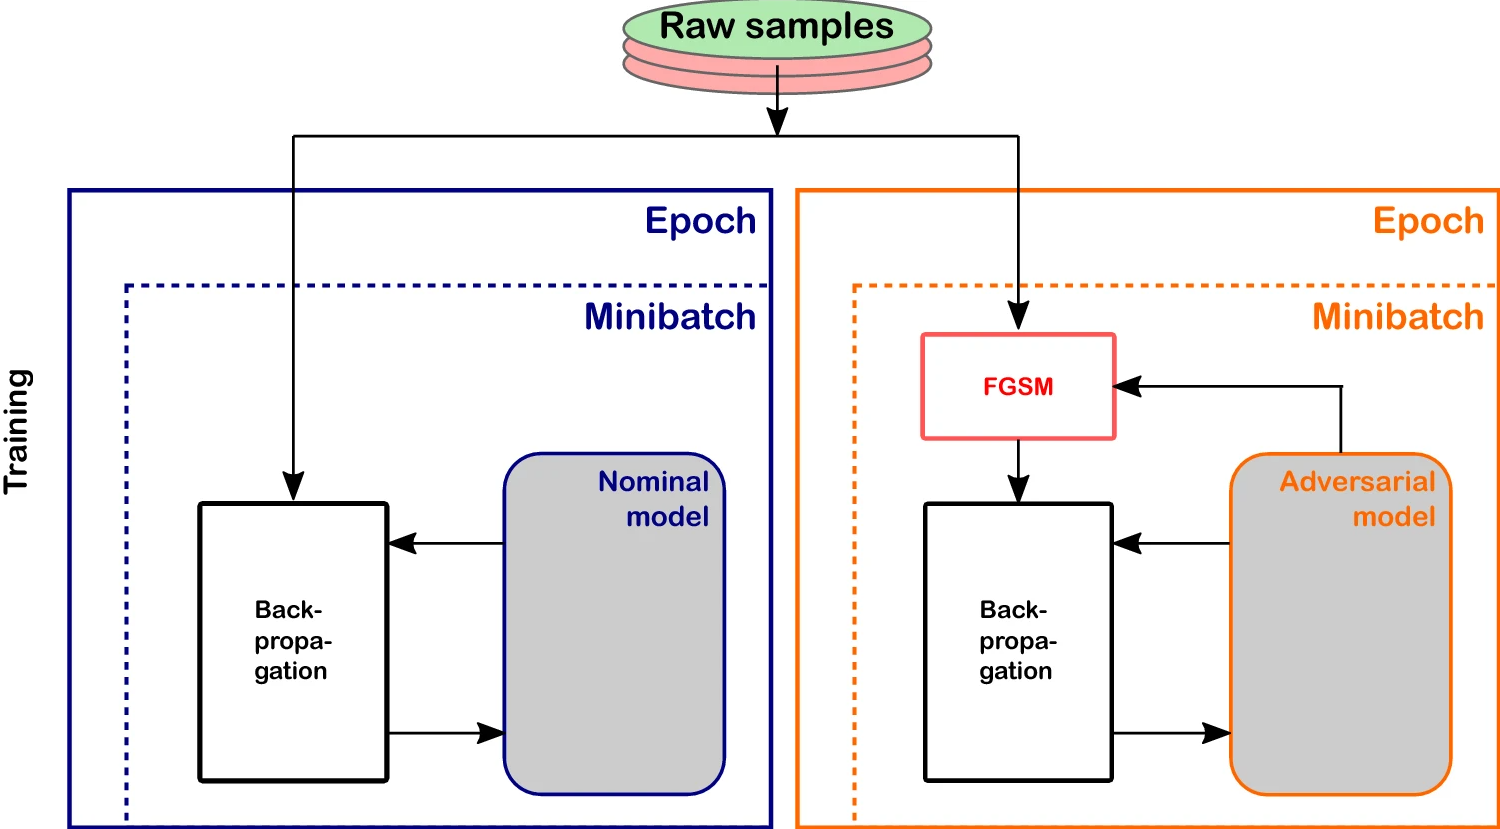
\includegraphics[width=0.8\linewidth]{media/adversarial_training.png}
    \caption{Comparison between nominal and adversarial training procedure for a neural network. The network on the right is trained on adversarial samples that are designed to fool the network, generated by the FGSM attack. By training on the adversarial examples, the network is less susceptible to adversarial attacks \cite{Stein2022}.}
    \label{fig:adversarial_training}
\end{figure}

In HEP, adversarial training reduces reliance on simulator-specific quirks and improves resilience to mismodelling. For example, if a tagger leans on a mismodelled feature, training with amplified versions of that mismatch pushes the network to learn more robust discriminants. This strategy was demonstrated by injecting slight perturbations into jet features during training — effectively simulating systematic shifts — and showed that the resulting tagger maintained high nominal performance while becoming significantly less vulnerable to such shifts \cite{Stein2022}. The adversarially-trained model coped better with variations in detector response and particle distribution, suggesting improved generalization to real data.

\section{The DeepJet Tagger}
\label{sec:DeepJet}

The DeepJet tagger represents a successful application of deep learning to a classic HEP problem by distinguishing heavy-flavour jets from light-quark or gluon jets. These taggers employ hierarchical neural-network architectures to combine information from many low-level inputs and produce a single probability for each flavour category. The key insight of DeepJet is to use as much information as possible about each jet, instead of relying on a hand-selected subset of inputs as previous algorithms did \cite{Bols_2020}. Earlier-generation taggers like CSV/DeepCSV used a fixed number of high-quality tracks and secondary vertices as input. In contrast, DeepJet forgoes a broad preselection of jet constituents; it ingests an extensive list of per-particle features – including charged and neutral particle-flow candidates, secondary vertex properties, and global jet attributes – and makes the neural network learn which features are important \cite{Bols_2020}.

\subsection{Candidate selection}

The candidate preselection is built on jets reconstructed using the particle-flow (PF) algorithm of CMS. Jets are clustered from PF candidates with the anti-$k_T$ algorithm that is based on the distance between constituents of the jet \cite{Tumasyan_2022}. The PF event reconstruction identifies and reconstructs individual particles (photons, electrons, muons, charged/neutral hadrons) by optimally combining information from all subdetectors \cite{Tumasyan_2022}. This provides a detailed list of charged and neutral particle candidates for each jet, along with any reconstructed secondary vertices from decays of long-lived particles.

All PF candidates associated with a jet – both charged and neutral – are used as inputs, supplemented by up to four secondary vertices and a set of global jet features. To maintain a fixed-size input representation, a maximum of 25 charged PF candidates and 25 neutral PF candidates are included per jet. This “no strict preselection” approach retains as much information as possible, avoiding the loss of potentially useful tracks that earlier methods discarded \cite{Bols_2020}.

\subsection{Architecture}

\begin{figure}[h]
    \centering
    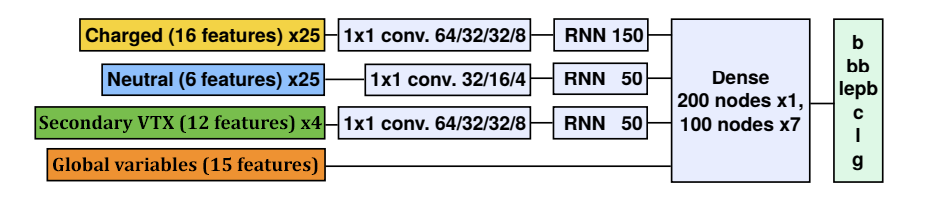
\includegraphics[width=1\linewidth]{media/deepJet_architecture.png}
    \caption{Illustration of the DeepJet architecture, adapted from \cite{Bols_2020} to fit the dataset (see \ref{sec:dataset}). Charged and neutral particle-flow
candidates, secondary vertices, and global variables are used as inputs to the tagger, which are processed by the hidden layers (white). The model outputs the probabilities for a jet to belong to one of the six jet classes.}
    \label{fig:deepjetArchitecture}
\end{figure}

The DeepJet Tagger takes 15 global input variables, 16 charged ParticleFlow (CPF) input variables for 25 candidates, 6 neutral ParticleFlow (NPF) input variables for 25 candidates and 12 secondary vertex (SV) input variables for 4 candidates, constituting 613 inputs per jet (see figure \ref{fig:deepjetArchitecture}). In the first stage, separate input streams are established for each type of low-level object: one for charged particles (tracks), one for neutral particles, and one for secondary vertices. Each stream passes through a stack of $1\times1$ convolutional layers with \textit{kernel size = 1} with bias parameters. These layers compute per-particle features without mixing information across particles, so each particle receives the same operation regardless of order \cite{Bols_2020}. Essentially, this track learns a representation for each track, each neutral, and each vertex input. Next, the outputs of these convolutional streams are fed into recurrent layers (LSTMs \cite{Goodfellow-et-al-2016}). The charged candidate LSTM uses 150 nodes, the neutral LSTM and secondary vertex LSTM each use 50 nodes. The LSTM outputs then are fed into a dense layer of 200 nodes followed by seven layers of 100 nodes each, using ReLU activation throughout. The final output layer is based on a softmax activation function and consists of six nodes, which are the model outputs for the six jet categories.